% Digital Logic Report Template
% Created: 2020-01-10, John Miller

%==========================================================
%=========== Document Setup  ==============================

% Formatting defined by class file
\documentclass[11pt]{article}

% ---- Document formatting ----
\usepackage[margin=1in]{geometry}	% Narrower margins
\usepackage{booktabs}				% Nice formatting of tables
\usepackage{graphicx}				% Ability to include graphics

%\setlength\parindent{0pt}	% Do not indent first line of paragraphs 
\usepackage[parfill]{parskip}		% Line space b/w paragraphs
%	parfill option prevents last line of pgrph from being fully justified

% Parskip package adds too much space around titles, fix with this
\RequirePackage{titlesec}
\titlespacing\section{0pt}{8pt plus 4pt minus 2pt}{3pt plus 2pt minus 2pt}
\titlespacing\subsection{0pt}{4pt plus 4pt minus 2pt}{-2pt plus 2pt minus 2pt}
\titlespacing\subsubsection{0pt}{2pt plus 4pt minus 2pt}{-6pt plus 2pt minus 2pt}

% ---- Hyperlinks ----
\usepackage[colorlinks=true,urlcolor=blue]{hyperref}	% For URL's. Automatically links internal references.

% ---- Code listings ----
\usepackage{listings} 					% Nice code layout and inclusion
\usepackage[usenames,dvipsnames]{xcolor}	% Colors (needs to be defined before using colors)

% Define custom colors for listings
\definecolor{listinggray}{gray}{0.98}		% Listings background color
\definecolor{rulegray}{gray}{0.7}			% Listings rule/frame color

% Style for Verilog
\lstdefinestyle{Verilog}{
	language=Verilog,					% Verilog
	backgroundcolor=\color{listinggray},	% light gray background
	rulecolor=\color{blue}, 			% blue frame lines
	frame=tb,							% lines above & below
	linewidth=\columnwidth, 			% set line width
	basicstyle=\small\ttfamily,	% basic font style that is used for the code	
	breaklines=true, 					% allow breaking across columns/pages
	tabsize=3,							% set tab size
	commentstyle=\color{gray},	% comments in italic 
	stringstyle=\upshape,				% strings are printed in normal font
	showspaces=false,					% don't underscore spaces
}

% How to use: \Verilog[listing_options]{file}
\newcommand{\Verilog}[2][]{%
	\lstinputlisting[style=Verilog,#1]{#2}
}




%======================================================
%=========== Body  ====================================
\begin{document}

\title{ELC 2137 Lab 10: 7-segment Display with Time-Division Multiplexing}
\author{Ashlie Lackey}

\maketitle


\section*{Summary}

Having previously created a 7-segment display with manual switching between digit displays, we know use a clock to display the digits simultaneously to the eye. By displaying the digit individually, but using a clock to display them at 100MHz, the eye perceives the individual displays lighting up as happening simultaneously to create a 4-digit 7-segment display. In accomplishing this, students gain skills in using synchronous design for sequential circuits, creating a parameterized counter-timer, and use of multiple counters to make a clock-driven 4-digit display. 

\section*{Q\&A}
\begin{enumerate}
  \item What are the three main “groups” of the RTL definition of sequential logic?
  
  The three main groups are state memory, next-state, and output logic.
  
  \item Copy Figure 10.3b onto your own paper (or do  it  electronically) and draw three  boxes around the components that belong to each group. Include your annotated figure  in your report.
  
  \begin{figure}[ht]\centering
  	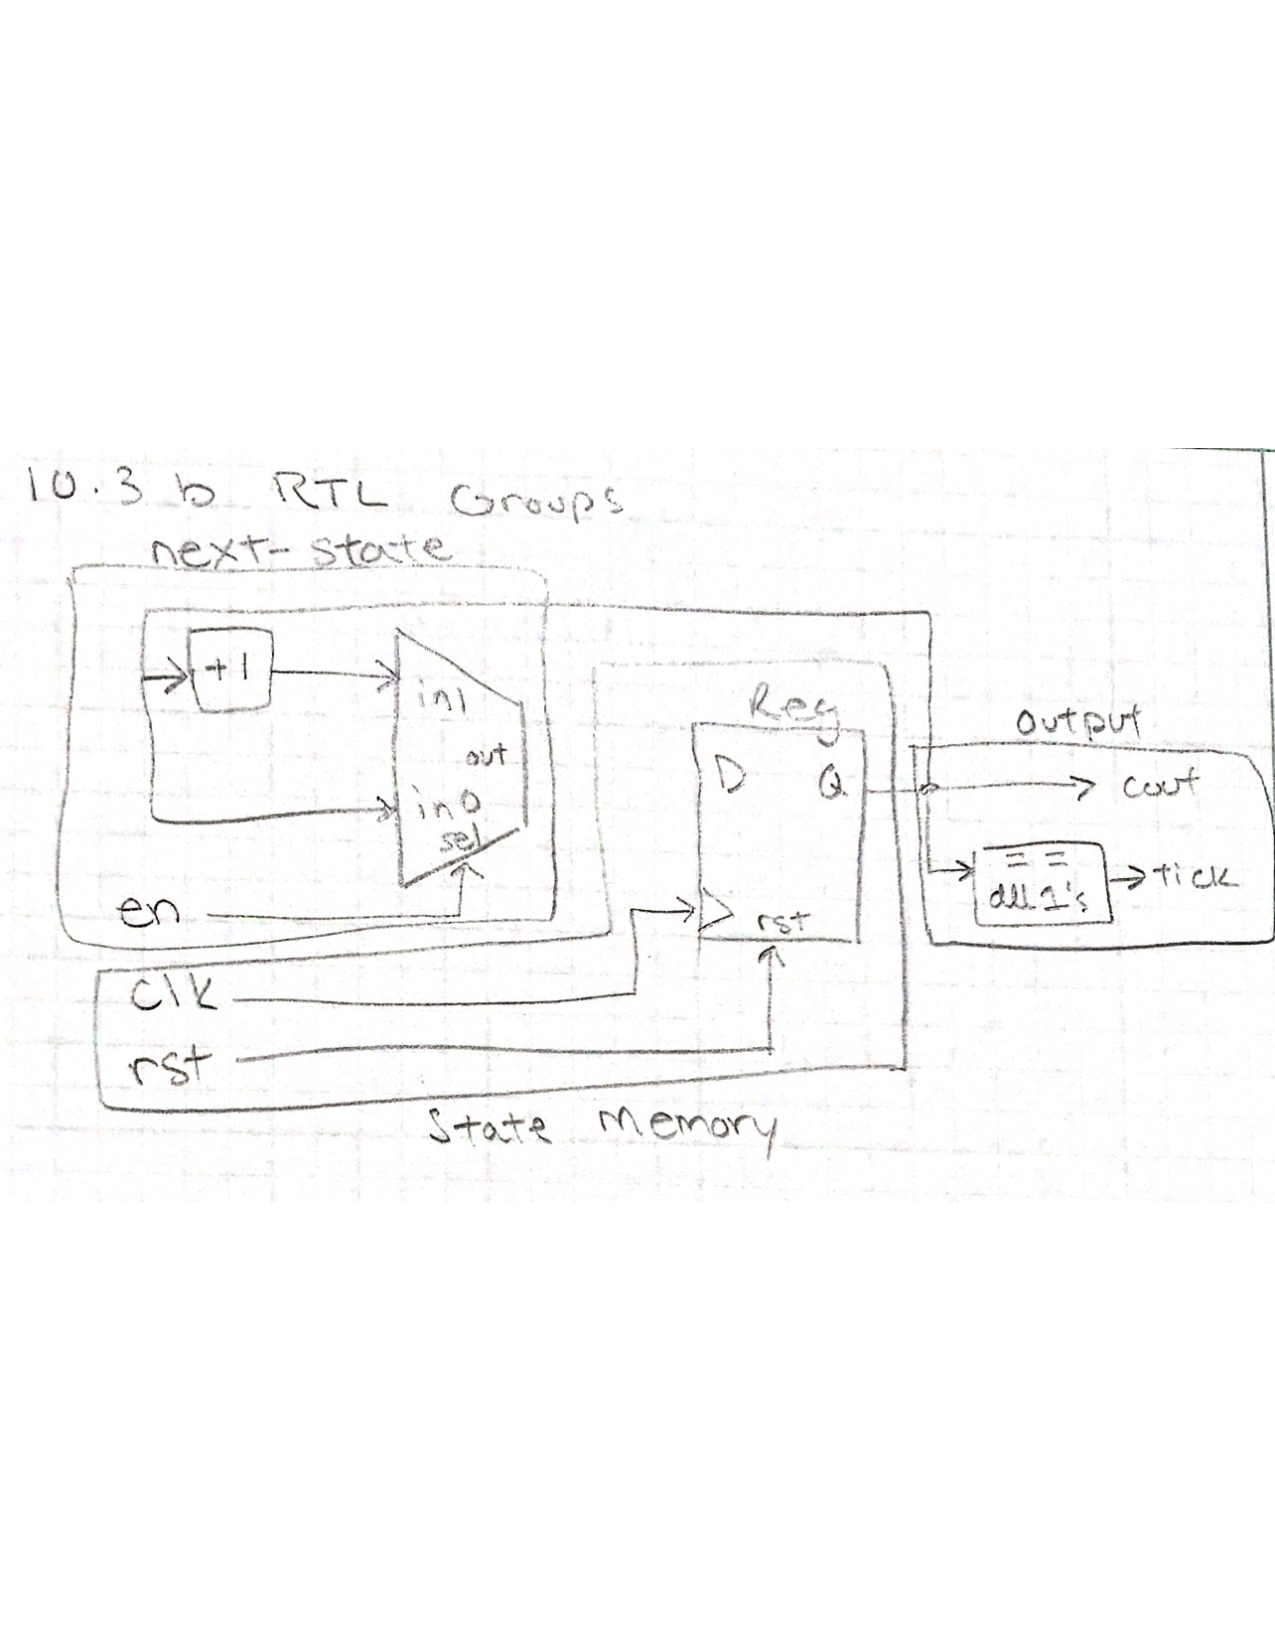
\includegraphics[width=1\textwidth]{rtl_groups}
  	\caption{\textit{10.3(b)} RTL Groups Schematic}
  	\label{fig:sim_with_table}
  \end{figure}
  \clearpage
  
  \item If instead of a counter, you wanted to make a shift register that moved the input  bits from right to left (low to high). What would you put on the line Qnext = /*???*/?
  
  Qnext = Q\_reg - 1'b1
  

\end{enumerate}

\section*{Results}
  
Expected results table, simulation waveforms, and schematic drawings are included in this portion of the report.

NOTE: The sseg4\_TDM testbench could not be configured correctly, so the ERT and Waveform are not included

\subsection*{Expected results tables}

\begin{table*}[ht]\centering
	\caption{\textit{counter\_test} expected results table}
	\label{ALU:tbl:alu_ERT}\medskip
	\begin{tabular}{l|rrrrrrrrrrrrr}
		Time (ns): & 0-5 & 5-7 & 7-10 & 10-15 & 15-20 & 20-25 & 25-30 & 30-35 & 35-40 & 40-45 & 45-50 &...\\
		\midrule
		clk & 0  & 1 & 1 & 0 & 1 & 0 & 1 & 0 & 1 & 0 & 1 & ... \\
		en & 0 & 0 & 0 & 1 & 0 & 1 & 0 & 1 & 0 & 1 & 0 & ...\\
		rst & 0 & 0 & 1& 0 & 0 & 0 & 0 & 0 & 0 & 0 & 0 & ... \\
		\midrule
		count & X & X & 0 & 0  & 1 & 1 & 2 & 2 & 3 & 3 & 0 & ... \\
		tick & X & X & 0 & 0 & 0 & 0 & 0 & 0 & 1 & 1 & 0& ... \\
		\bottomrule
	\end{tabular}
\end{table*}

\begin{table*}[ht]\centering
	\caption{\textit{counter\_test} expected results table}
	\label{ALU:tbl:alu_ERT}\medskip
	\begin{tabular}{l|rrrrrrr}
		Time (ns): & 0-2 & 2-5 & 5-10 & ... & 1000005-2000000 & 2000000-2621435 & 2621435-3000005\\
		\midrule
		data(hex) & 1234 & 1234 123 && ... & 1234  & 1234 & 1234  \\
		hex\_dec & 0 & 0 & 0 & ... & 1 &  0 & 0\\
		sign & 0 & 0 & 0 & ... & 0 &  1 & 1 \\
		reset & 0 & 1 & 0 & ... & 0 & 0 & 0  \\
		clock & 0 & 0 & 5 & ...  \\
		\midrule
		seg (hex) & X & 19 & 19 & ... & 19 & 19 & 30 \\
		dp & 1 & 1 & 1 & ... & 1 & 1 & 1 \\
		an (hex)& X & e & e & ... & e & e & d \\
		\bottomrule
	\end{tabular}
\end{table*}

\clearpage
 
\subsection*{Simulation Waveforms}
\begin{figure}[ht]\centering
	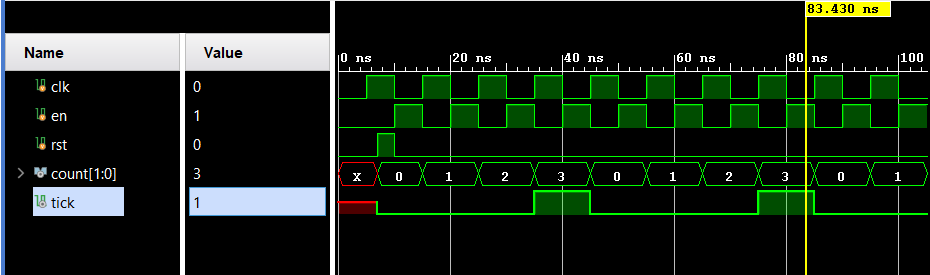
\includegraphics[width=1.1\textwidth]{counter_test}
	\caption{\textit{counter testbench} Simulation Waveform}
	\label{fig:sim_with_table}
\end{figure}

\begin{figure}[ht]\centering
	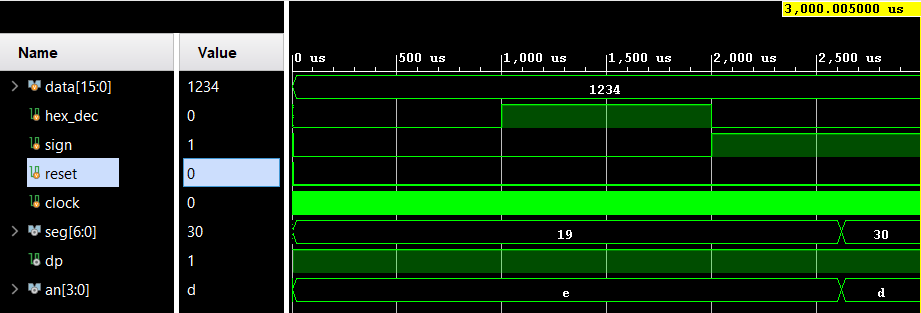
\includegraphics[width=1.1\textwidth]{sseg4_test}
	\caption{\textit{sseg4\_TDM testbench} Simulation Waveform}
	\label{fig:sim_with_table}
\end{figure}

\clearpage

\subsection*{Schematics}

\begin{figure}[ht]\centering
	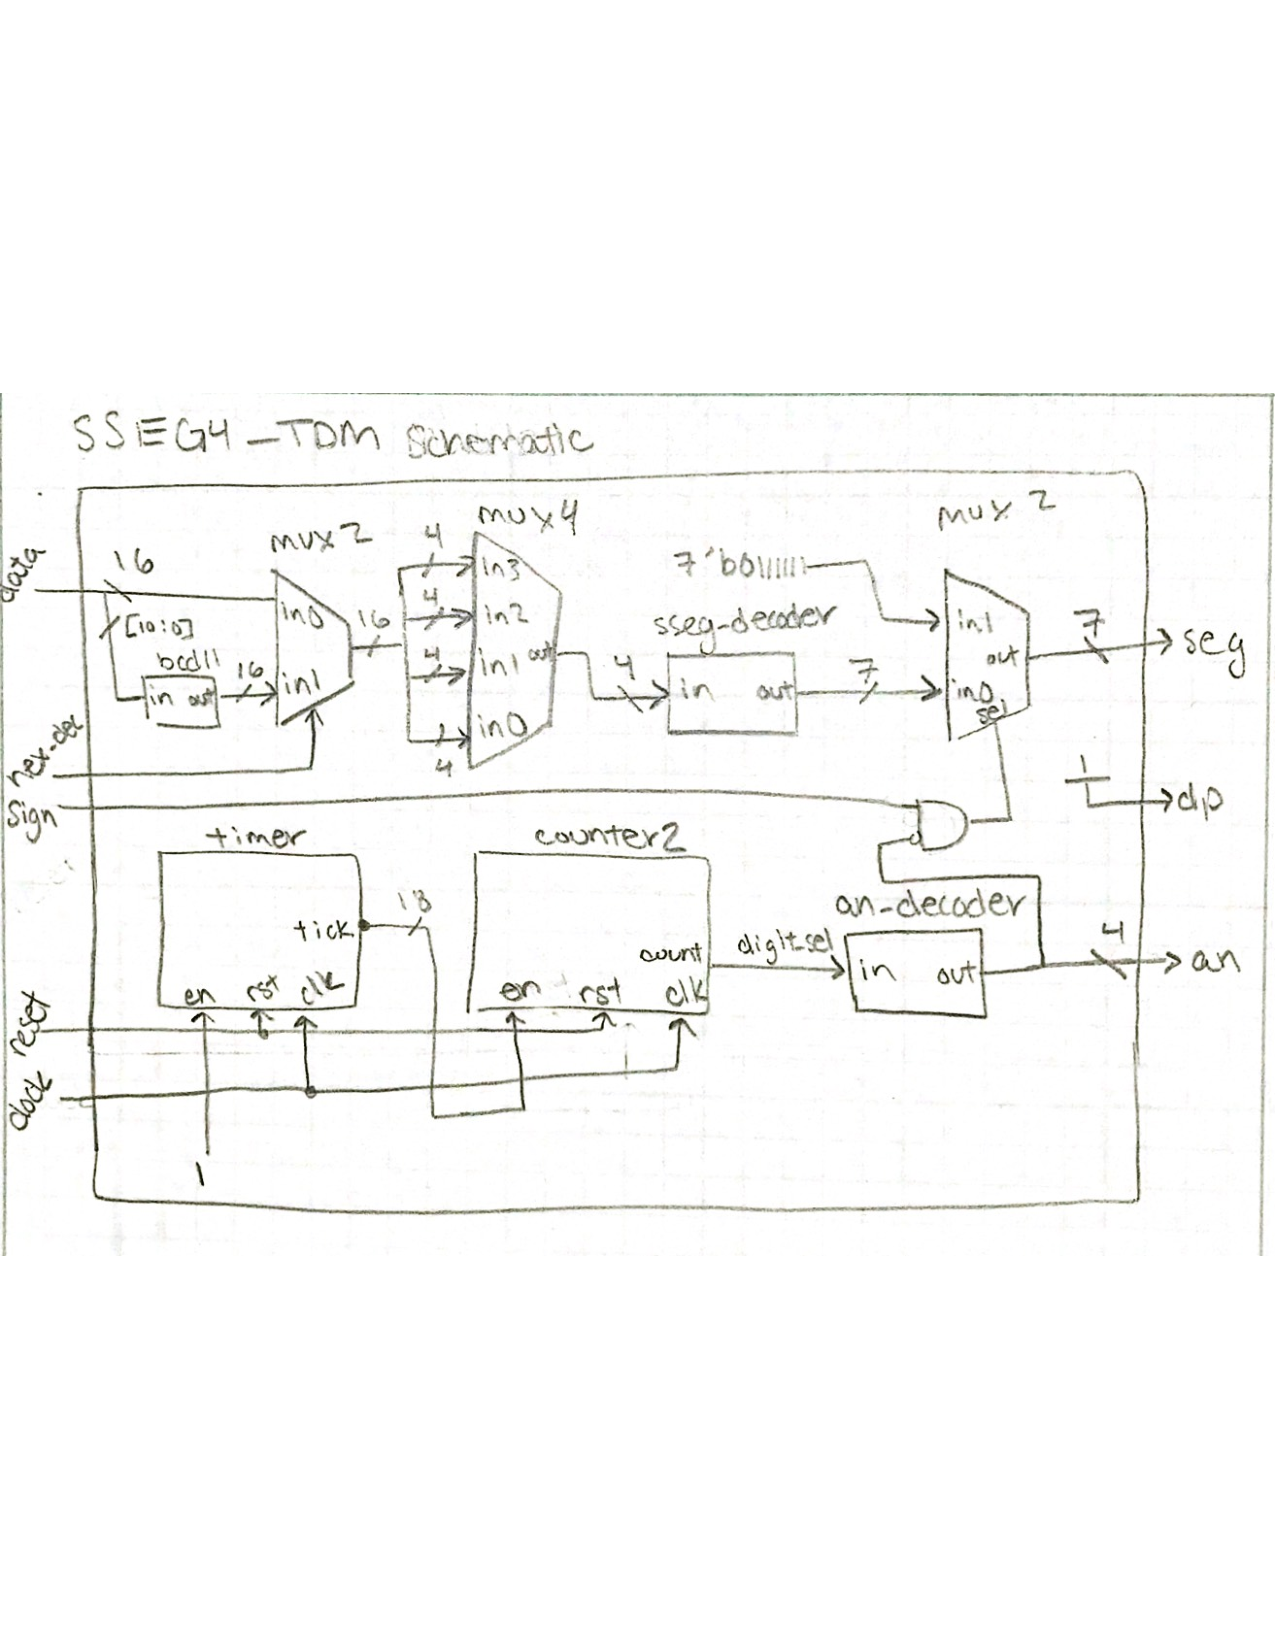
\includegraphics[width=1\textwidth]{sseg4_sch}
	\caption{\textit{sseg4\_TDM} Module Schematic}
	\label{fig:sim_with_table}
\end{figure}

\begin{figure}[ht]\centering
	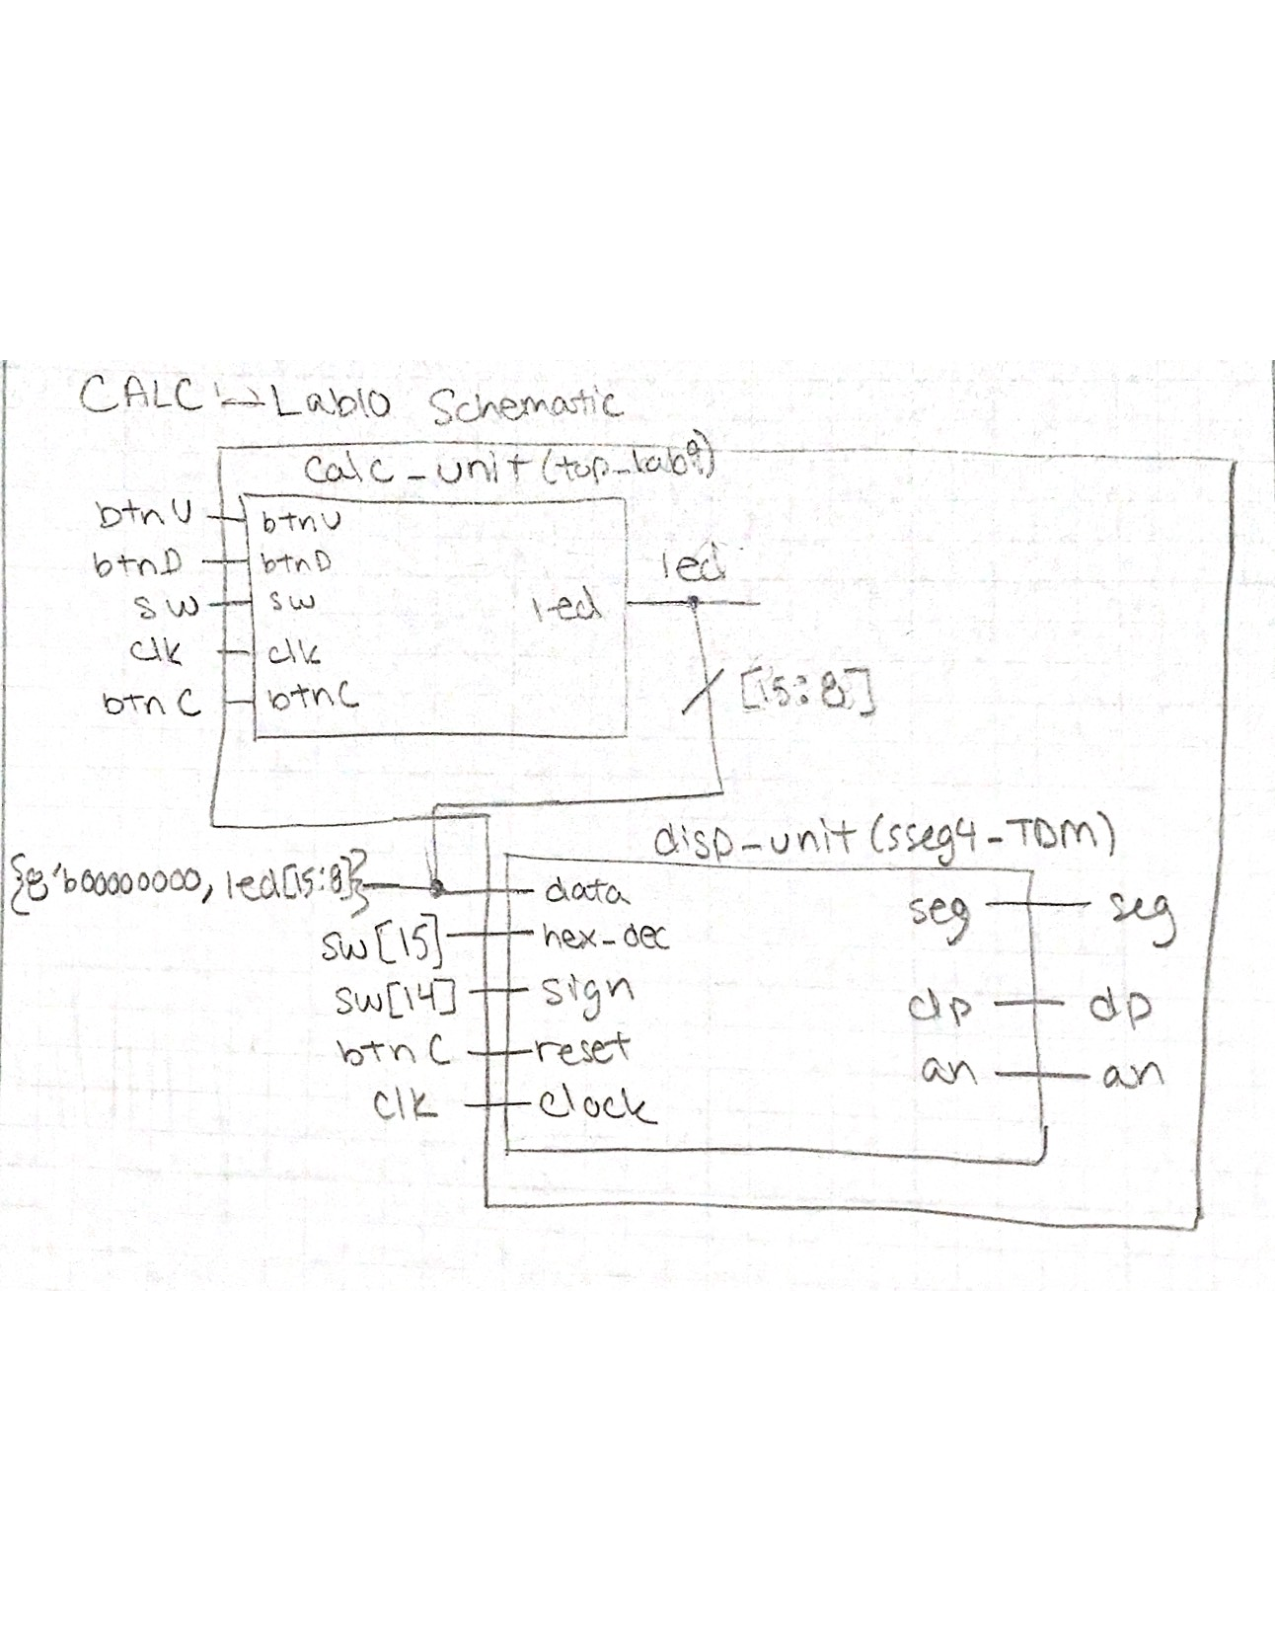
\includegraphics[width=1\textwidth]{calc10_sch}
	\caption{\textit{calc\_lab10} Module Schematic}
	\label{fig:sim_with_table}
\end{figure}

\clearpage

\section*{Code}
.

\begin{lstlisting}[style=Verilog,caption=Counter Verilog Code,label=code:ex ]
`timescale 1ns / 1ps
// Ashlie Lackey, ELC 2137, 2020 -04 -08
module counter #( parameter N=1)
	(
	input clk, rst, en,
	output [N-1:0] count ,
	output tick
	);
	
	// internal signals
	reg [N-1:0] Q_reg , Q_next ;
	
	// register ( state memory )
	always @ ( posedge clk , posedge rst )
	begin
		if (rst)
			Q_reg <= 0;
		else
			Q_reg <= Q_next;
	end
	// next - state logic
	always @ *
	begin
		if (en)
			Q_next = Q_reg + 1'b1; //increase by one
		else
			Q_next = Q_reg; // no change
	end
	
	// output logic
	assign count = Q_reg ;
	assign tick = ( Q_reg =={ N{1'b1} } ) ? 1'b1 : 1'b0;
endmodule // counter
\end{lstlisting}

\begin{lstlisting}[style=Verilog,caption= sseg4\_TDM Verilog Code,label=code:ex ]
`timescale 1ns / 1ps
// Ashlie Lackey, ELC 2137 , 2020 -04 -13

module sseg4_TDM(
	input [15:0] data,
	input hex_dec, sign, reset, clock,
	output reg [6:0] seg,
	output reg dp,
	output reg [3:0] an);
	
	wire [17:0] count_dontcare; 
	wire tick_out;
	counter #(.N(18)) timer(.clk(clock),.en(1), .rst(reset), 
		.count(count_dontcare), .tick(tick_out) );
	
	wire [1:0] digit_sel;
	wire tick_dontcare;
	counter #(.N(2)) counter2(.clk(clock),.en(tick_out), .rst(reset),
		.count(digit_sel), .tick(tick_dontcare) );
	
	wire [15:0] bcd11out ;
	bcd11 TDM_bcd11 (.B(data [10:0]) , .Boutfinal(bcd11out) ) ;
	
	wire [15:0] mux2_1_out ;
	mux2 #(.N(16)) TDM_mux2_1 (.in0(data [15:0]), .in1(bcd11out), .sel(
		hex_dec), .out(mux2_1_out) );
	
	wire [3:0] mux4_out;
	mux4 TDM_mux4 (.in0 mux2_1_out [3:0]) , .in1( mux2_1_out [7:4]), .in2 (
		mux2_1_out [11:8]) , .in3( mux2_1_out [15:12]), .sel(digit_sel) , .out(mux4_out) ) ;
	
	wire [6:0] sseg_decoder_out ;
	sseg_decoder TDM_decode (. num ( mux4_out ) , . sseg ( sseg_decoder_out ) ) ;
	
	wire [3:0] decoder_out ;
	an_decode an_decode_TDM (. in ( digit_sel ) , . out ( decoder_out ) ) ;
	
	wire mux22_in ;
	assign mux22_in = ~ decoder_out [3] & sign ;
	mux2 #(.N(7)) TDM_mux2_2 (.in0( sseg_decoder_out ) , .in1(7'b0111111 ) , .sel ( 	mux22_in ) , . out ( seg ) ) ;
	
	assign dp = 1;
	assign an = decoder_out ;
endmodule
\end{lstlisting}

\begin{lstlisting}[style=Verilog,caption= calc\_lab10 Verilog Code ,label=code:ex ]
`timescale 1ns / 1ps
// Ashlie Lackey, ELC 2137, 2020 -04 -08
module calc_lab10(input btnU, btnD,
	input [15:0] sw,
	input clk, btnC,
	output [15:0] led,
	output dp ,
	output [3:0] an,
	output [6:0] seg);
	
	
	top_lab9 calc_unit(.btnU(btnU), .btnD(btnD),.sw(sw),.clk(clk), .btnC(btnC),.led(led));
	
	sseg4_TDM disp_unit(.data({8'b00000000, led[15:8]}),.hex_dec(sw[15]), .sign(sw[14]),
		.reset(btnC), .clock(clk),.seg(seg),.dp(dp),.an(an));
endmodule
\end{lstlisting}

\begin{lstlisting}[style=Verilog,caption= counter\_test testbench Verilog Code,label=code:ex ]
`timescale 1ns / 1ps
// Ashlie Lackey, ELC 2137, 2020 -04 -08
module counter_test();
	reg clk , en , rst;
	wire [1:0] count;
	wire tick;
	
	counter #(.N(2)) c(.clk(clk),.en(en), .rst(rst), .count(count), .tick(tick) );
	// clock  runs  continuously
	always  begin
		clk = ~clk; #5;
	end
	// this  block  only  runs  once
	initial  begin
		clk=0; en=0; rst =0; #7;
		rst = 1; #3; //  reset
		en = 1; rst = 0; #5;
		en = 0; #5;
		en = 1; #5;
		en = 0; #5;
		en = 1; #5;
		en = 0; #5; 
		en = 1; #5;
		en = 0; #5; 
		en = 1; #5;
		en = 0; #5; 
		en = 1; #5;
		en = 0; #5; 
		en = 1; #5;
		en = 0; #5; 
		en = 1; #5;
		en = 0; #5; 
		en = 1; #5;
		en = 0; #5;
		en = 1; #5;  
	$finish;
	end
endmodule
\end{lstlisting}

\begin{lstlisting}[style=Verilog,caption= sseg4\_TDM\_test Code,label=code:ex ]
`timescale 1ns / 1ps
// Ashlie Lackey, ELC 2137, 2020 -04 -08
module sseg4_TDM_test();
	reg [15:0] data;
	reg hex_dec, sign, reset, clock;
	wire [6:0] seg;
	wire dp;
	wire [3:0] an;
	
	sseg4_TDM TDM_test(.data(data), 
	.hex_dec(hex_dec), .sign(sign), .reset(reset), 
	.clock(clock),.seg(seg),.dp(dp),.an(an));
	
	// clock  runs  continuously
	always  begin
		clock = ~clock; #5;
	end 
	
	
	initial begin
		data = 16'h1234; clock = 0; reset =0; #2;
		reset = 1; #3; //  reset
		reset = 0; hex_dec = 0; sign = 0; #1000000; 
		hex_dec = 1; sign = 0; #1000000;
		hex_dec = 0; sign = 1; #1000000;
	$finish;
	end

endmodule
\end{lstlisting}

\end{document}

	
	
	
	


	
